%File: formatting-instructions-latex-2024.tex
%release 2024.0
\documentclass[letterpaper]{article} % DO NOT CHANGE THIS
\usepackage{aaai24}  % DO NOT CHANGE THIS
\usepackage{times}  % DO NOT CHANGE THIS
\usepackage{helvet}  % DO NOT CHANGE THIS
\usepackage{courier}  % DO NOT CHANGE THIS
\usepackage[hyphens]{url}  % DO NOT CHANGE THIS
\usepackage{graphicx} % DO NOT CHANGE THIS
\urlstyle{rm} % DO NOT CHANGE THIS
\def\UrlFont{\rm}  % DO NOT CHANGE THIS
\usepackage{natbib}  % DO NOT CHANGE THIS AND DO NOT ADD ANY OPTIONS TO IT
\usepackage{caption} % DO NOT CHANGE THIS AND DO NOT ADD ANY OPTIONS TO IT
\frenchspacing  % DO NOT CHANGE THIS
\setlength{\pdfpagewidth}{8.5in}  % DO NOT CHANGE THIS
\setlength{\pdfpageheight}{11in}  % DO NOT CHANGE THIS
%
% These are recommended to typeset algorithms but not required. See the subsubsection on algorithms. Remove them if you don't have algorithms in your paper.
% \usepackage{algorithm}
% \usepackage{algorithmic}

%
\usepackage{amsthm}
\usepackage{amsmath}
\newtheorem{theorem}{Theorem}
\newtheorem{definition}{Definition}
\usepackage[inkscapelatex=false]{svg}
\usepackage[ruled,boxed]{algorithm2e}
\makeatletter
\g@addto@macro{\@algocf@init}{\SetKwInOut{Parameter}{Parameter}}
% \g@addto@macro{\@algocf@init}{\SetKwInOut{Require}{Require}}
\makeatother
\usepackage{amsfonts}
% \usepackage{utfsym}
\usepackage{bbding}
\usepackage{booktabs}
% \usepackage[]{footmisc}

% These are are recommended to typeset listings but not required. See the subsubsection on listing. Remove this block if you don't have listings in your paper.
\usepackage{newfloat}
\usepackage{listings}
\DeclareCaptionStyle{ruled}{labelfont=normalfont,labelsep=colon,strut=off} % DO NOT CHANGE THIS
\lstset{%
	basicstyle={\footnotesize\ttfamily},% footnotesize acceptable for monospace
	numbers=left,numberstyle=\footnotesize,xleftmargin=2em,% show line numbers, remove this entire line if you don't want the numbers.
	aboveskip=0pt,belowskip=0pt,%
	showstringspaces=false,tabsize=2,breaklines=true}
% \floatstyle{ruled}
% \newfloat{listing}{tb}{lst}{}
% \floatname{listing}{Listing}
% %
% Keep the \pdfinfo as shown here. There's no need
% for you to add the /Title and /Author tags.

% DISALLOWED PACKAGES
% \usepackage{authblk} -- This package is specifically forbidden
% \usepackage{balance} -- This package is specifically forbidden
% \usepackage{color (if used in text)
% \usepackage{CJK} -- This package is specifically forbidden
% \usepackage{float} -- This package is specifically forbidden
% \usepackage{flushend} -- This package is specifically forbidden
% \usepackage{fontenc} -- This package is specifically forbidden
% \usepackage{fullpage} -- This package is specifically forbidden
% \usepackage{geometry} -- This package is specifically forbidden
% \usepackage{grffile} -- This package is specifically forbidden
% \usepackage{hyperref} -- This package is specifically forbidden
% \usepackage{navigator} -- This package is specifically forbidden
% (or any other package that embeds links such as navigator or hyperref)
% \indentfirst} -- This package is specifically forbidden
% \layout} -- This package is specifically forbidden
% \multicol} -- This package is specifically forbidden
% \nameref} -- This package is specifically forbidden
% \usepackage{savetrees} -- This package is specifically forbidden
% \usepackage{setspace} -- This package is specifically forbidden
% \usepackage{stfloats} -- This package is specifically forbidden
% \usepackage{tabu} -- This package is specifically forbidden
% \usepackage{titlesec} -- This package is specifically forbidden
% \usepackage{tocbibind} -- This package is specifically forbidden
% \usepackage{ulem} -- This package is specifically forbidden
% \usepackage{wrapfig} -- This package is specifically forbidden
% DISALLOWED COMMANDS
% \nocopyright -- Your paper will not be published if you use this command
% \addtolength -- This command may not be used
% \balance -- This command may not be used
% \baselinestretch -- Your paper will not be published if you use this command
% \clearpage -- No page breaks of any kind may be used for the final version of your paper
% \columnsep -- This command may not be used
% % \newpage -- No page breaks of any kind may be used for the final version of your paper
% \pagebreak -- No page breaks of any kind may be used for the final version of your paperr
% \pagestyle -- This command may not be used
% \tiny -- This is not an acceptable font size.
% \vspace{- -- No negative value may be used in proximity of a caption, figure, table, section, subsection, subsubsection, or reference
% \vskip{- -- No negative value may be used to alter spacing above or below a caption, figure, table, section, subsection, subsubsection, or reference

\setcounter{secnumdepth}{0} %May be changed to 1 or 2 if section numbers are desired.

% The file aaai24.sty is the style file for AAAI Press
% proceedings, working notes, and technical reports.
%

% Title

% Your title must be in mixed case, not sentence case.
% That means all verbs (including short verbs like be, is, using,and go),
% nouns, adverbs, adjectives should be capitalized, including both words in hyphenated terms, while
% articles, conjunctions, and prepositions are lower case unless they
% directly follow a colon or long dash
% \iffalse
% \title{AAAI Press Formatting Instructions \\for Authors Using \LaTeX{} --- A Guide}
% \author{
%     %Authors
%     % All authors must be in the same font size and format.
%     Written by AAAI Press Staff\textsuperscript{\rm 1}\thanks{With help from the AAAI Publications Committee.}\\
%     AAAI Style Contributions by Pater Patel Schneider,
%     Sunil Issar,\\
%     J. Scott Penberthy,
%     George Ferguson,
%     Hans Guesgen,
%     Francisco Cruz\equalcontrib,
%     Marc Pujol-Gonzalez\equalcontrib
% }
% \affiliations{
%     %Afiliations
%     \textsuperscript{\rm 1}Association for the Advancement of Artificial Intelligence\\
%     % If you have multiple authors and multiple affiliations
%     % use superscripts in text and roman font to identify them.
%     % For example,

%     % Sunil Issar\textsuperscript{\rm 2},
%     % J. Scott Penberthy\textsuperscript{\rm 3},
%     % George Ferguson\textsuperscript{\rm 4},
%     % Hans Guesgen\textsuperscript{\rm 5}
%     % Note that the comma should be placed after the superscript

%     1900 Embarcadero Road, Suite 101\\
%     Palo Alto, California 94303-3310 USA\\
%     % email address must be in roman text type, not monospace or sans serif
%     proceedings-questions@aaai.org
% %
% % See more examples next
% }
% \fi

%Example, Single Author, ->> remove \iffalse,\fi and place them surrounding AAAI title to use it
\iffalse
\title{My Publication Title --- Single Author}
\author {
    Author Name
}
\affiliations{
    Affiliation\\
    Affiliation Line 2\\
    name@example.com
}
\fi

% \iffalse
%Example, Multiple Authors, ->> remove \iffalse,\fi and place them surrounding AAAI title to use it
\title{H-ensemble: an Information Theoretic Approach to \\Reliable Few-Shot Multi-Source-Free Transfer}
\author {
    % Authors
    Yanru Wu \textsuperscript{\rm 1}, %\thanks{Corresponding author},
    Jianning Wang \textsuperscript{\rm 2},
    Weida Wang \textsuperscript{\rm 1},
    Yang Li \textsuperscript{\rm 1}\footnote{Corresponding author.} %\textsuperscript{\dag}
}
\affiliations {
    % Affiliations
    \textsuperscript{\rm 1}Tsinghua Shenzhen International Graduation School, Tsinghua University\footnote{Yanru Wu, Weida Wang and Yang Li are from the Shenzhen Key Laboratory of Ubiquitous Data Enabling, SIGS, Tsinghua.}\\
    \textsuperscript{\rm 2}School of Computer Science and Engineering, Harbin Institute of Technology, Shenzhen\\
    % \textsuperscript{\rm 3}Tsinghua Shenzhen International Graduation School, Tsinghua University\\
    \{wu-yr21, wangwd19\}@mails.tsinghua.edu.cn, wangjianning@stu.hit.edu.cn, yangli@sz.tsinghua.edu.cn
}
% \fi



\begin{document}

\maketitle

\begin{abstract}
Multi-source transfer learning is an effective solution to data scarcity by utilizing multiple source tasks for the learning of the target task. However, access to source data and model details is limited in the era of commercial models, giving rise to the setting of \textit{multi-source-free} (MSF) transfer learning that aims to leverage source domain knowledge without such access. As a newly defined problem paradigm, MSF transfer learning remains largely underexplored and not clearly formulated. In this work, we adopt an information theoretic perspective on it and propose a framework named \textit{H-ensemble}, which dynamically learns the optimal linear combination, or ensemble, of source models for the target task, using a generalization of maximal correlation regression. The ensemble weights are optimized by maximizing an information theoretic metric for transferability. Compared to previous works, H-ensemble is characterized by: 1) its adaptability to a novel and realistic MSF setting for few-shot target tasks, 2) theoretical reliability, 3) a lightweight structure easy to interpret and adapt. Our method is empirically validated by ablation studies, along with extensive comparative analysis with other task ensemble and transfer learning methods. We show that the H-ensemble can successfully learn the optimal task ensemble, as well as outperform prior arts.
%\wangedit: In the age of commercial models, the challenge of accessing source data and model intricacies has spotlighted the emergent concept of \textit{multi-source-free} (MSF) transfer learning, aiming to leverage source domain knowledge without direct access. Though rich in potential, the MSF transfer learning paradigm remains in its infancy and demands clearer formulation. Addressing this gap, our study offers an information-theoretic lens to MSF transfer learning, culminating in the introduction of the \textit{H-ensemble} network. This framework dynamically amalgamates the optimal linear blend of source models for the target task via a generalized maximal correlation regression. Distinguishing features of our H-ensemble include its debut under the novel MSF setting tailored for few-shot target tasks, its theoretical robustness, and a nimble, interpretable structure conducive to adaptations. Comprehensive ablation studies and comparative analyses against prevailing ensemble and transfer learning methodologies underscore the efficacy of our approach, revealing the H-ensemble's adeptness at discerning optimal task ensembles and its demonstrable superiority over existing techniques.

\end{abstract}

\section{Introduction}

The scarcity of annotated data is a principal challenge to machine learning algorithms in a variety of real-world scenarios, where transfer learning has emerged as an effective remedy, harnessing information and insights from well-established source tasks to augment data-deficient domains \citep[see][]{perkins1992transfer, weiss2016survey, zhuang2020comprehensive}. Historically, transfer learning has centered on a singular source-task and target-task relationship. However, the spotlight is gradually shifting towards multi-source transfer learning, capitalizing on multiple source tasks to facilitate the training of the target task \citep[see][]{sun2015survey}. A variety of works have contributed to both the theoretical foundation and practical algorithms on this topic.
Yet, the trend of decentralization and growing privacy concerns have impeded access to source data, particularly when compared to the models they've nurtured \citep{feng2021kd3a}. This evolving landscape underscores the need for the novel paradigm of \textit{multi-source-free} (MSF) transfer learning \citep{fang2022source}.

%\wangedit: In machine learning applications, a prominent bottleneck is the scarcity of annotated data. In various real-world contexts, obtaining reliable labeled data is often challenging due to the steep costs of data acquisition and human annotation. Transfer learning has emerged as a potent remedy, harnessing information and insights from well-established source tasks to augment data-deficient domains \citep[see][]{perkins1992transfer, weiss2016survey, zhuang2020comprehensive}.



%\wangedit: Historically, transfer learning has centered on a singular source-task and target-task relationship. However, the spotlight is gradually shifting towards multi-source transfer learning, capitalizing on multiple source tasks to bolster the training of a single target task \citep[see][]{sun2015survey}. Numerous contributions have enriched this field with foundational theories and practical algorithms. Yet, the trend of decentralization and heightened privacy concerns has impeded access to source data, particularly when compared to the models they've nurtured \citep{feng2021kd3a}. This evolving landscape underscores the need for the novel paradigm of \textit{multi-source-free} transfer learning \citep{fang2022source}.




MSF transfer learning, sometimes referred to as MSF domain adaptation \citep{han2023discriminability}, entails transferring knowledge from multiple sources to a target task without accessing source data, as depicted in Fig. \ref{fig:setup}.
% This setting is branched from normal multi-source transfer \citep[see][also briefly introduced in the section of related works]{sun2015survey} and is gaining emphasis recently, as well-trained source models are much easier to obtain than the data they are trained on due to the trend of decentralization and privacy protection \citep{feng2021kd3a}.
% As illustrated in \ref{fig:setup}, in multi-source-free transfer people have a set of trained source models but no source data, where the goal is to leverage them for the target task.
Despite not being clearly defined in most previous papers and still largely underexplored, MSF transfer has been explored by several works these years. Preliminary efforts centered around simple strategies like averaging source models or reducing the problem to single source-free transfers, by source selection using empirical validations or transferability metrics \citep[e.g.][]{yang2023pick}. Contemporary research has pivoted towards sophisticated model ensembles, assigning weights to sources based on perceived importance. For instance, approaches range from correlating source relevance to the target \citep{lee2019learning}, to conditional entropy minimization \citep{ahmed2021unsupervised}, and even leveraging source-similarity and class-relationship perception modules for weight determination \citep{dong2021confident, han2023discriminability}.
Beyond these linear ensemble techniques, some researchers also introduced auxiliary models to endow cross-domain capabilities \citep{li2022source}.
% For example, \citeauthor{lee2019learning} (\citeyear{lee2019learning}) weighted the sources by measuring their relativity to the target with maximal correlation; \citeauthor{ahmed2021unsupervised} (\citeyear{ahmed2021unsupervised}) had their weights given by pseudo-labeling and then minimizing a conditional entropy term;  \citeauthor{dong2021confident} (\citeyear{dong2021confident}) and \citeauthor{han2023discriminability} (\citeyear{han2023discriminability}) both used a source-similarity-based transferability perception module and a class-relationship-aware proxy discriminability perception to jointly determine the source weights. Apart from linear ensemble of source models, \citeauthor{li2022source} (\citeyear{li2022source}) introduced an auxiliary general model trained on sources as a multi-task model to provide cross-domain ability.

\begin{figure}[ht]
    \centering
    \centerline{\includesvg[width=0.8\columnwidth]{figures/setup2.svg}}
    % \includegraphics[width=\columnwidth]{}
    \caption{\textbf{Problem Setting of Multi-Source-Free Transfer Learning.} The transfer to the target task is based on the source models (whose access in our redefined MSF setting is also restricted) trained on the inaccessible source data. }
    \label{fig:setup}
\end{figure}

%\wangedit: Labeled interchangeably as multi-source-free domain adaptation \citep{han2023discriminability}, this approach entails transferring knowledge from multiple sources to a target task without accessing source data, as depicted in Fig. \ref{fig:setup}. Despite its nascent stage, a handful of explorations have tackled multi-source-free transfer. Preliminary efforts centered around simple strategies like averaging source models or condensing the challenge to source-free transfers using empirical validations or transferability metrics \citep[e.g.][]{yang2023pick}. Contemporary research has pivoted towards sophisticated model ensembles, assigning weights to sources based on perceived importance. For instance, approaches range from correlating source relevance to the target \citep{lee2019learning}, to conditional entropy minimization \citep{ahmed2021unsupervised}, and even leveraging source-similarity and class-relationship perception modules for weight determination \citep{dong2021confident, han2023discriminability}. Beyond these linear ensemble techniques, some researchers have pioneered auxiliary models to endow cross-domain capabilities \citep{li2022source}.

\subsection{Motivation}

While these methods have their merits, %supported by rigorous experiments and sound logic,
they still present three distinct limitations.
Firstly,
they mainly evaluate the source importance as an independent characteristic of each source instead of viewing them as a
%\scout{entity}
whole,
% which may cause
% %\scout{neglection}
% negligence of the possible interaction when ensembling models.
neglecting the likely interaction effects when combining.
% This problem will be solved in our work by optimizing the weight vector as a single variable.
Secondly, these works
% \footnote{All except \citeauthor{lee2019learning} in \citeyear{lee2019learning}, which didn't clearly state or formulate the multi-source-free setting.}
focus on the unsupervised MSF transfer,
% with an unsupervised target, where the target input can be fully acquired but without label annotation.
while a more common setting of data scarcity in practice is \textit{few-shot} learning, where we can only access a few of the target data but with labels \citep{wang2020generalizing}. Thirdly, most of them hinge on accessing intermediate layer outputs or necessitate tuning of source models, which tend to become inaccessible in the era of proprietary large models. Also, despite their effectiveness, these transfer algorithms have quite complicated methodologies, making them hard to interpret or adapt.

%\wangedit: While these methodologies have their merits, underpinned by rigorous experiments and sound logic, they present three distinct limitations. Firstly, they often evaluate source importance in isolation, overlooking potential synergies when combining models. Secondly, these works\footnote{All except \citeauthor{lee2019learning} in \citeyear{lee2019learning}, which didn't clearly state or formulate the multi-source-free setting.} only focus on the unsupervised multi-source-free transfer, while a more common setting of data scarcity in practice is \textit{few-shot} learning, where we can only access a few of the target data but with their labels \citep{wang2020generalizing}. Lastly, these methods often hinge on accessing intermediate layer outputs or necessitate retraining of source models. In the age of proprietary large models, such access is increasingly elusive. Moreover, the intricate designs of these transfer techniques compromise their interpretability and adaptability.

As a solution to these issues, we focus on the few-shot MSF transfer challenge, proposing a novel transfer framework tailored to this setting.
Given the scarcity of target samples and the inaccessibility of source details, we base our methodology on the optimization of features instead of the analysis of input data as other works did.
Specifically, following the idea of linear source ensemble, we define the target feature as a weighted combination of transferred features and introduce an information theoretic metric, \textit{H-score}, to gauge the quality of this synthesis, which can be alternatively interpreted as the transferability of the whole source model ensemble. The optimal source weights will then be simply determined by maximizing this metric, leveraging the robustness of H-score under few-shot settings as well as its computational efficiency and theoretical reliability \citep{huang2019information}.
%Our subsequent target task resolution hinges on a generalized maximal correlation regression.
Our derived target generalizes the maximal correlation regression (MCR) by replacing its feature by an ensemble of source feature extractors and modifying the model accordingly.
%Considering its emphasis on feature ensemble and H-score based optimization, this framework is named as \textit{H-ensemble}.
A detailed explanation of the underlying theoretic basis and intuition of H-ensemble framework will be presented in the Methodology section, showing that: 1) under the maximal correlation framework, the weights maximizing our adapted H-score are theoretically optimal for the target task; 2) the resulting optimal question is of a benign form and can be reliably solved by gradient descend based algorithms.

%\wangedit: Addressing these issues, our work focuses on the few-shot multi-source-free transfer challenge, presenting a novel framework tailored to this setting. Given the paucity of target samples and inaccessible source specifics, we emphasize feature optimization over traditional input data analysis. Our approach, grounded in linear source ensemble ideology, frames the target feature as a weighted amalgamation of transferred features. We then employ an H-score metric to gauge the quality of this synthesis. Interpreted through the lens of source model ensemble transferability, we optimize source weights to maximize this metric. Our subsequent target task resolution hinges on a generalized maximal correlation regression, leveraging the H-score's robustness in few-shot scenarios, combined with computational efficiency and theoretical rigor \citep{huang2019information}. We will later explain in detail the underlying theoretic basis and intuition of this framework in the Methodology section, showing that: 1) under the maximal correlation framework, the weights maximizing our adapted H-score are theoretically optimal for the target task; 2) the resulting optimal question is of a benign form and can be reliably solved by gradient descend based algorithms.


% Specifically, the transferred feature is a weighted combination of feature extracted by source models, and an H-score based metric is employed to measure its quality.


% task. its formula directly derived from maximal correlation analysis

    % \begin{itemize}
    %     \item[-] optimize the source weight vector as a whole variable;
    %     \item[-] touch on another prevalent setting in both real-world and machine learning research referred to as \textit{few-shot} learning ;
    %     \item[-] propose a information theoretic transfer framework that is both theoretically reliable and easy to interpret/adapt with a simple and intuitive model structure.
    % \end{itemize}

% \noindent Moreover, we also tightened the source-free restriction so that we have no access to either source data or internal details of source models,
% % as it is more frequently the case nowadays with the thriving of closed large models provided by commercial companies.
% % impose a source-free condition that requires us to perform MSFTL without source data or further training or accessing the internal details of source models,



% which is a rising scenario .
% A detailed formulation of our problem setting and comparison with other works will be presented in the Problem Definition section.
% We then inherit the ideas of MSFTL and go on to propose our methodology under the setting we defined.
% We then inherit the ideas of MSFTL and propose our methodology under the setting we defined.


% \begin{table*}[htb]
%     \renewcommand{\arraystretch}{1.2}
%     \centering
%     \begin{tabular}{c c c c c}
%         \toprule
%          \textbf{Setting} &  \textbf{Multiple Sources} & \textbf{No Source Data} & \textbf{No Source Model Details} & \textbf{Target} \\
%          \midrule
%          FS Transfer & \usym{2717} & \usym{2717} & \usym{2717} & Few-shot \\
%          UDA &  \usym{2717} & \usym{2717} & \usym{2717} & Unsupervised \\
%          MSDA &  \usym{2713} & \usym{2717} & \usym{2717} & Unsupervised \\
%          MSFDA  &  \usym{2713} & \usym{2713} & \usym{2717} & Unsupervised \\
%          FSMSF Transfer (Ours)  &  \usym{2713} &  \usym{2713} &  \usym{2713} & Few-shot \\
%          \bottomrule

%     \end{tabular}
%     \caption{ Our setting is of the most strict source-free restriction. Listed from top to bottom are traditional Few-Shot transfer learning \citep[FS Transfer, see][]{wang2020generalizing}, Unsupervised Domain Adaptation \citep[UDA, see][]{hoffman2018cycada}, Multi-Source Domain Adaptation \citep[MSDA, see][]{peng2019moment}, Multi-Source-Free Domain Adaptation \citep[MSFDA, see][]{ahmed2021unsupervised} and ours (FEMSF Transfer).}
%     \label{tab:setting}
% \end{table*}







\begin{table*}[htb]
\setlength{\tabcolsep}{4pt}
    \renewcommand{\arraystretch}{1.2}
    \centering
    \begin{tabular}{c c c c c}
        \toprule
         \textbf{Setting} &  \textbf{Multi-Source} & \textbf{No Source Data} & \textbf{No Source Model Details} & \textbf{Target} \\
         \midrule
         Few-Shot transfer \citep[]{wang2020generalizing} & \XSolidBrush & \XSolidBrush & \XSolidBrush & Few-shot \\
         Unsupervised DA \citep[]{hoffman2018cycada} &  \XSolidBrush & \XSolidBrush & \XSolidBrush & Unsupervised \\
         Multi-Source DA \citep[]{peng2019moment} &  \Checkmark & \XSolidBrush & \XSolidBrush & Unsupervised \\
         Multi-Source-Free DA \citep[]{ahmed2021unsupervised}  &  \Checkmark & \Checkmark & \XSolidBrush & Unsupervised \\
         Few-Shot Multi-Source-Free Transfer (Ours)  &  \Checkmark &  \Checkmark &  \Checkmark & Few-shot \\
         \bottomrule
    \end{tabular}
    \caption{\textbf{Comparison across Relative Problem Settings,} involving the aspects of whether there are multi-sources, no source data, no source model details, and different target learning approaches. The abbreviation `DA' represents domain adaptation, `\Checkmark' represents obtaining the corresponding aspects, while `\XSolidBrush' the opposite. Among all settings, ours is relatively restrictive.}
    \label{tab:setting}
\end{table*}

% \sout{With a large range of available sources and limitation in computational resources, it is necessary to have a methodology that can efficiently and reliably utilize multiple sources for boosting learning of given target task.}

\subsection{Contributions}
In this paper, we propose an information theoretic MSF transfer framework named \textit{H-ensemble}, where the source models are assembled using a generalization of MCR, and the source weights are obtained by maximizing an H-score based metric.
% in this work we define a new problem scenario of multi-source transfer called few-shot multi-source-free transfer. Under this setting, we propose an information theoretic multi-source transfer framework based on the \underline{M}aximal \underline{c}orrelation regression \underline{N}etwork and source task \underline{E}nsemble with the \underline{W}eights determined by optimizing the fused feature quality estimated by \underline{H}-score metric, which is named as McNEW-H.
Our contributions mainly lie in three aspects:


\begin{itemize}
    \item[a)] We formulate the few-shot MSF transfer problem mathematically using a source-free setting that is more common in practical scenarios.

        % \sout{\textbf{i.} where a higher-level source-free setting than previous works is employed as more frequently confronted in practical scenarios. \textbf{ii.} emphasize tackle of the data scarcity problem }

    \item[b)] An efficient and theoretically reliable framework derived from maximal correlation regression is introduced for MSF transfer. The framework is designed to be lightweight and easy to interpret and adapt, possible to serve as a \textit{plug-in} module.
    %TODO: lightweight?

    \item[c)] We present both theoretical guarantee and experimental support to the effectiveness of our methodology.

    % We provide both theoretical and experimental evidence for the effectiveness of our methodology by maximizing the correlation between the target and source models.

\end{itemize}

\section{Related Works}
\subsection{Maximal Correlation Regression and H-Score}\label{sec:H-score}

 Maximal correlation regression (MCR) network \citep{xu2020maximal} refers to a specially designed network trained based on the optimization of feature quality by maximizing H-score. Here, H-score is a metric determining whether certain features are informative for the task  \citep[more formally introduced by][]{bao2019information}\footnote{The H-score introduced by Bao et al. is actually the one-sided form of the score in MCR (both firstly defined by Huang et al. in 2019). They are also differed in their definition of variables and optimal objects.}. Its derivation is rooted in the maximal correlation interpretation of deep neural networks \citep{huang2019universal}, where given the extracted features, the formula of H-score is actually the optimal network performance under an information theoretic measurement. Previous work also extended H-score to a transferability metric and verified its effectiveness with extensive experiments \citep{bao2019information, ibrahim2022newer}, suggesting the potential of H-score in transfer learning.

Notably, as the basis of both MCR network and H-score, maximal correlation analysis originates from the works of Hirschfeld, Gebelein and Renyi \citep{hirschfeld1935connection, gebelein1941statistische, renyi1959measures} and has been followed and further explored by a broad spectrum of successive work. A detailed overview of maximal correlation analysis can be found given by \citeauthor{huang2019universal} (\citeyear{huang2019universal}).

% By definition, H-score is a metric assessing the informativeness of features for a task \citep[formally introduced by][]{bao2019information} derived from the maximal correlation interpretation of deep neural networks \citep{huang2019universal}.
% Maximal Correlation Regression (MCR) network \citep{xu2020maximal} is trained by maximizing the H-score of features. Previous works also extended H-score as a transferability metric and demonstrated its effectiveness through extensive experiments \citep{bao2019information, ibrahim2022newer}. Foundational to both MCR network and H-score, maximal correlation analysis originates from the works of Hirschfeld, Gebelein, and Renyi \citep{hirschfeld1935connection, gebelein1941statistische, renyi1959measures}. A comprehensive overview of this analysis is provided by \citeauthor{huang2019universal} (\citeyear{huang2019universal}).

% \subsection{Few-Shot Learning}

% Few-shot Learning (FSL) is proposed to tackle the learning problems with small data set.
% \citep{wang2020generalizing}


\subsection{Multi-Source Transfer Learning}\label{sec:multisource}

% Transferring using multiple sources is a long-proposed idea. Elementary works on this topic include naive multi-source transfer by concatenating all source feature extractors together for finetuning \citep{christodoulidis2016multisource} and theoretical works as in \citep{crammer2008learning, mansour2008domain, ben2010theory, tong2021mathematical}.

% Well-developed algorithms can be mainly divided into three types. Re-weighting approaches use different strategies to estimate source importance and assign the weights accordingly \citep[][]{sun2011two, lee2019learning}. Source selection methods propose multi-source transferability metrics to elect the best combination \citep{agostinelli2022transferability}. Boosting-based solutions adapt ensemble learning techniques to transfer learning \citep[][]{huang2012boosting, xu2012multi, fang2019adapted}. More of this topic can be found in related papers and surveys \citep[e.g.][]{sun2015survey}.

Multi-source transfer learning, a well-established concept, encompasses approaches like naive multi-source transfer by feature extractor concatenation \citep{christodoulidis2016multisource} and theoretical explorations \citep{crammer2008learning, mansour2008domain, ben2010theory, tong2021mathematical, chen2023algorithm}. Contemporary algorithms can be classified into three main categories: re-weighting approaches that estimate and assign source importance \citep{sun2011two, lee2019learning, shui2021aggregating}; source selection methods using transferability metrics to identify optimal combinations \citep{agostinelli2022transferability}; and boosting-based solutions that apply ensemble learning techniques to transfer learning \citep{huang2012boosting, xu2012multi, fang2019adapted}. Further insights on this topic are available in related surveys, such as \citep{sun2015survey}.

\section{Problem Definition}

\subsection{Setting Comparison to Previous Works}

Based on the change of settings mentioned in the Introduction section, there are mainly three terms to emphasize in our setting: multi-source, source-free and few-shot. Specially, to distinguish from previous notions, source-free is categorized into source-data-free and source-model-free. We compare few-shot MSF transfer with previous settings in these four aspects and summarize the main divergence in Table~\ref{tab:setting}.

% \begin{itemize}
%     \item \textbf{Multi-Source:} Transfer to the target task using multiple sources.
%     \item \textbf{Source-Free:} No access to either source data or internal details (structures/weights) of source models. Specifically, the latter indicates that any modification of source models or acquisition of information other than the output feature is not allowed.
%     \item \textbf{Few-Shot:} Target task only contains a few samples with supervised information.
% \end{itemize}

 \begin{table}[!ht]
     \renewcommand{\arraystretch}{1.2}
    \centering
    \begin{tabular}{c |c }
        \toprule
        \textbf{Notation} & \textbf{Meaning}\\
        \midrule
        $S_j$; $T$ & Source/Target Task\\
        $d_{S_j}$; $d_T$& Source/Target Class Number\\
         % $d_f$ & United feature dimension\\
     $N_{S_j}$; $N_T$ & Source/Target Data Size \\
         $D_{S_j} = \{(x_{S_j}^i, y_{S_j}^i)\}_{i = 1}^{N_{S_j}}$ & Source Data \\
         $D_T = \{(x_T^i, y_T^i)\}_{i = 1}^{N_T}$ & Target Data \\
          \bottomrule
    \end{tabular}
    \caption{\textbf{Notation.} We omit $\{\cdot\}_{j=1}^M$ for simplification.}
    \label{tab:notation}
\end{table}

\subsection{Mathematical Formulation}


Consider the transfer learning setting with $M$ source tasks $\{S_j\}_{j=1}^M$ and a target task $T$, we list the main notations in Table~\ref{tab:notation}.  For simplification, we assume that the sources and target tasks share the same input space $X$ and all tasks are classification problems.\footnote{This assumption is without loss of generality, for in most cases,
% one may easily preprocess the model input to any desired size
model inputs can be mapped to any size by preprocessing (e.g. image resizing, pooling, certain embedding layers, etc.),
% , and classification is still one of the most common task types in today's machine learning researches.
and classification is one of the most representative tasks in machine learning.}
% The learned source models are thus of the form $\theta_{S_j}: X \to \mathbb{R}^{d_{S_j}}$, and the problem goal will be to obtain the target model $\theta_T: X \to \mathbb{R}^{d_{T}}$.

Notably, in our setting we have no access to source data $D_{S_j}$ and only partial access to target data $D_T$, so here $N_{S_j} = 0$, $N_T = k \times d_T$ for a $k$-shot MSF transfer.\footnote{$k$ samples for each of the $d_T$ classes}
For the source model consisting of a backbone feature extractor $\boldsymbol{f}_{S_j}: X \to \mathbb{R}^{d_f}$ and a classification head $\boldsymbol{g}_{S_j}: \mathbb{R}^{d_f} \to \mathbb{R}^{d_{S_j}}$ ($d_f$ denotes the feature dimension)\footnote{$d_f$ is set to the same across all tasks considering that we could add a fully connected layer to derive any output dimension.}, where the source-free restriction leaves the detailed model structure unknown.

% We use the notation $D_{S_j} = \{(x_{S_j}^i, y_{S_j}^i)\}_{i = 1}^{N_{S_j}}$ for the data on source task $S_j$ , and $D_T = \{(x_T^i, y_T^i)\}_{i = 1}^{N_T}$ for the data on target task $T$,
% where $N_{S_j}$ and $N_T$ are the size of the source and target data.


In computation, we estimate the distribution $P^T_{X}$, $P^T_{Y}$ of target data $x_T$, $y_T$ with empirical distribution $\hat P^T_{X}$, $\hat P^T_{Y}$:

\begin{equation}
\hat P_{X}^T (x)= \frac{1}{N_T}\sum_{i=1}^{N_T}\mathbb{I}\{x_T^i=x\}; \hat P_{Y}^T (y)= \frac{1}{N_T}\sum_{i=1}^{N_T}\mathbb{I}\{y_T^i=y\},
\label{py}
\end{equation}

\noindent where $\mathbb{I}\{\cdot\}$ is the indicator function \citep{feller1991introduction}. Similarly, the conditional distribution of $x_T$ given $y_T$ $P^T_{X|Y}$ is estimated by its empirical distribution $\hat P^T_{X|Y}$:

\begin{equation}
\hat P^T_{X|Y} (x|y)= \frac{\sum_{i=1}^{N_T}\mathbb{I}\{x_T^i=x,y_T^i=y\}}{\sum_{i=1}^{N_T}\mathbb{I}\{y_T^i=y\}}.
\label{pxy}
\end{equation}

When estimating the underlying distributions with empirical distributions of samples, Eqns. (\ref{py}) and (\ref{pxy}) may be poorly defined and intractable for most target task types due to the high dimension of input $x$. However, this problem can be avoided, as in our framework we only need to compute the expectation of features over these distributions.
% of some elementary functions of features.

The goal of few-shot MSF problem is that, by utilizing the partially accessible data and black-box source models only, find the optimal parameters $\boldsymbol{\theta}_T$ that minimizes certain divergence $\mathcal L$ between the real conditional distribution $P^T_{Y|X}$ and the approximated $P^{(\boldsymbol{\theta}_T)}_{Y|X}$, \textit{i.e.},

\begin{equation}
    \boldsymbol{\theta}^*_T = arg\min_{\boldsymbol{\theta}_T} \mathcal L(P^{(\boldsymbol{\theta}_T)}_{Y|X}, P^T_{Y|X}).
    \label{definition}
\end{equation}

\begin{figure*}
    \centering
    \centerline{\includesvg[width=2\columnwidth]{figures/framework-neo.svg}}
    % 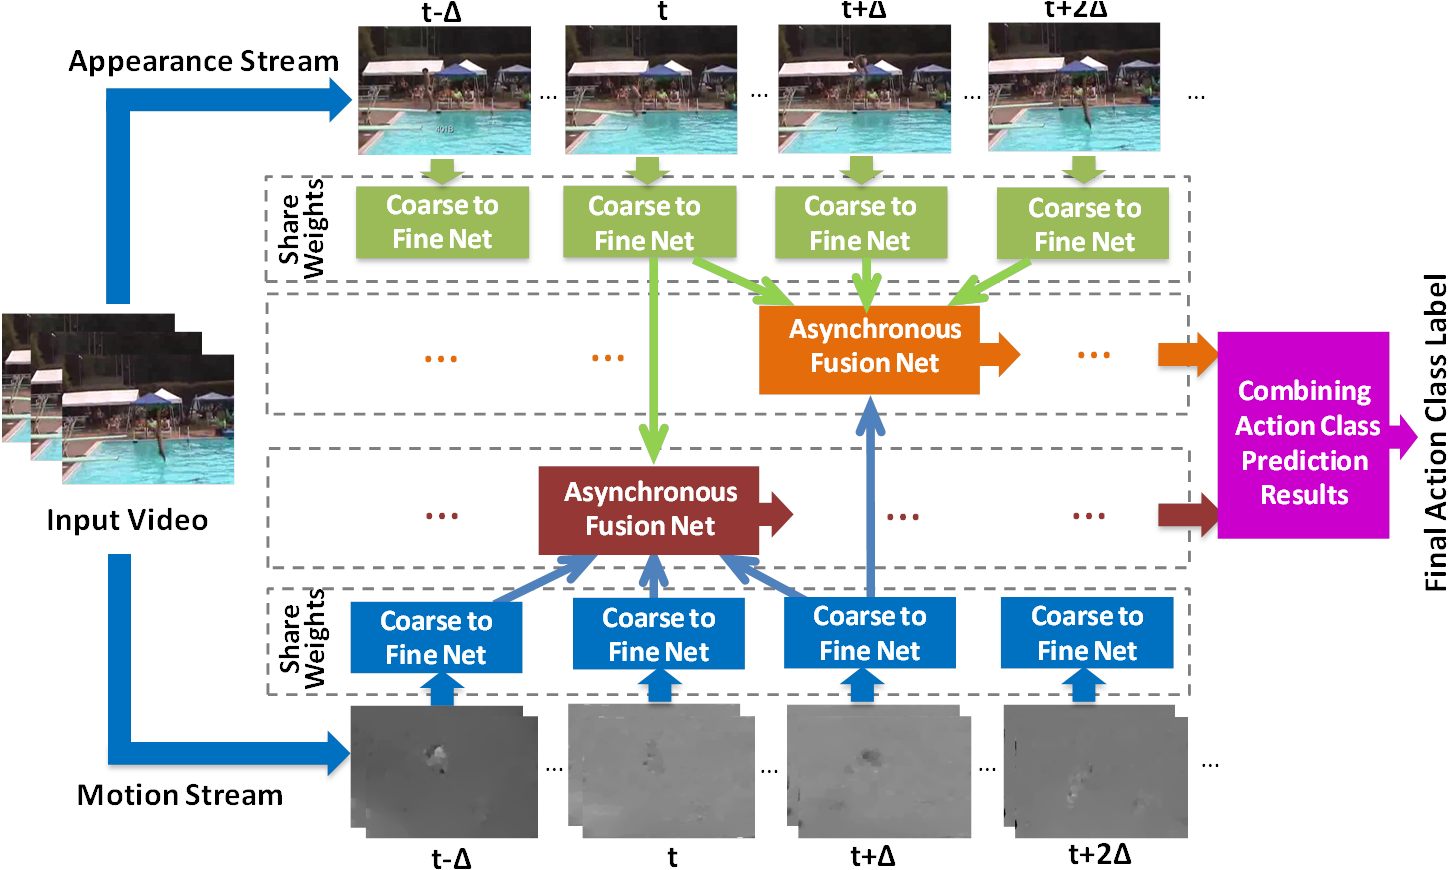
\includegraphics[width=2\columnwidth]{figures/framework.png}
    \caption{\textbf{Framework of H-Ensemble.} The framework consists of three modules. The target data firstly flow into Target Feature Extractor. Then the Weight Optimizer will utilize the outputs of source feature extractors and target label to derive the optimal source weight $\boldsymbol{\alpha}$, which makes the parameter in deriving target feature. Finally the Target Classifier will be trained and used together with the extractor for test according to a generalization of maximal correlation regression (MCR).}
    \label{fig:framework}
\end{figure*}



\section{Methodology}

Following the analysis in the Motivation section, we model the target feature extractor $\boldsymbol{f}_T$  by a weighted combination of source feature extractors $\boldsymbol{f}_{S_j}$:

\begin{equation}
    \begin{aligned}
        \boldsymbol{f}_T = \sum_{j=1}^M \alpha_j \cdot \boldsymbol{f}_{s_j}, \ \sum_{j=1}^M \alpha_j = 1 .
    \end{aligned}
    \label{targetfeature}
\end{equation}

We then need to efficiently evaluate target features to guide the optimization of weights $\boldsymbol{\alpha}$, where the maximal correlation analysis (MCA) is introduced. In MCA, a neural network is viewed as a feature extractor $\boldsymbol{f}$ and a classifier $\boldsymbol{g}$, and the informativeness of features extracted by $\boldsymbol{f}$ can be estimated by H-score.

Leveraging the robustness of H-score under few-shot settings as well as its computational efficiency and theoretical reliability, we use H-score as the feature quality measurement and set up the transfer framework under the same theory scheme as a generalization of MCR. Following previous works \citep{xu2020maximal}, the divergence $\mathcal L$ in Eqn. (\ref{definition}) is defined as variational chi-squared divergence:
\begin{equation}
    \mathcal L(\boldsymbol{\theta}) = \sum_x P_X(x) \sum_y \frac{[P^{(\boldsymbol{\theta})}_{Y|X} (y|x) - P_{Y|X} (y|x)]^2}{P_Y(y)}.
\end{equation}

We illustrate our MSF transfer framework H-ensemble in Fig. \ref{fig:framework} and introduce each module in the sections below, showing how the divergence $\mathcal L$ is minimized.

\subsection{Multi-Source-Free Transfer}


% We decompose each of the source models $\theta_{S_j}: X \to R^{d_{S_j}}$ into two parts: the feature extractor $\boldsymbol{f}_{S_j}: X \to R^{d_f}$ and the classifier $\boldsymbol{g}_{S_j}: R^{d_f} \to R^{d_{S_j}}$. Here $d_f$ denotes the feature dimension, which is set to the same across all tasks considering that we could use a fully connected layer to derive any output dimension with ease.

Overall, the MSF transfer framework follows the generalized MCR\citep{xu2020maximal} network and has two modules, feature extractor $\boldsymbol{f}_T = \sum_{j=1}^M \alpha_j \cdot \boldsymbol{f}_{s_j}$ and classifier $\boldsymbol{g}_T$ derived using MCR training mode as below. The approximated conditional distribution is defined as

% Overall, the MSF transfer framework is constructed by generalizing the MCR network, where we follow MCR  \citep{xu2020maximal} in splitting the target model as feature extractor $\boldsymbol{f}_T$ and classifier $\boldsymbol{g}_T$, with the former given by $\boldsymbol{f}_T = \sum_{j=1}^M \alpha_j \cdot \boldsymbol{f}_{s_j}$ and the latter derived using MCR training mode as below. The approximated conditional distribution is defined as

\begin{equation}
    P^{(\boldsymbol{\theta_T})}_{Y|X} (y|x) = P^T_Y(y) (1+\boldsymbol{f}_T^{\rm T}(x)\boldsymbol{g}_T(y)).
\end{equation}

% \noindent The above $\alpha_j$ denotes the weight for the $j$-th source feature extractor that should sum up to 1. The definition and optimization of the source weight $\alpha$ will be later introduced in detail in the following sections.

Specifically, given input data $x \sim P^T_X$, the features extracted by source models are $\boldsymbol{f}_{s_j}(x)$. To simplify the deduction, we assume that $\mathbb{E}_{P^T_X}[\boldsymbol{f}_{s_j}(x)] = 0$ and $\mathbb{E}_{P^T_X}[\boldsymbol{f}_{s_j}(x)\cdot \boldsymbol{f}_{s_j}(x)^{\rm T}] = \mathbf{I}$ for all $j$, as a normalization layer could be efficiently added to extractors. Subsequently, $\boldsymbol{f}_T$ is also a normalized feature with $\mathbb{E}_{P^T_X}[\boldsymbol{f}_{T}(x)] = 0$ and $\mathbb{E}_{P^T_X}[\boldsymbol{f}_{T}(x)\cdot \boldsymbol{f}_{T}(x)^{\rm T}] = \mathbf{I}$. After deriving the target feature extractor $\boldsymbol{f}_T$, the optimal target classifier $\boldsymbol{g}_T$ minimizing $\mathcal L(\boldsymbol{\theta}_T)$ can be directly calculated by generalizing MCR to a multiple extractor combination scenario.

\begin{theorem}
    Given feature extractors of function form $\boldsymbol{f}_{i}(x)$, $i \in \{1,\dots, n\} $ and the linearly combined feature extractor $\boldsymbol{f}(x) = \sum_{i=1}^n \alpha_i \cdot \boldsymbol{f}_i(x)$, where $\mathbb{E}_{P_X}[\boldsymbol{f}_i(x)] = 0$, $\mathbb{E}_{P_X}[\boldsymbol{f}_i(x)\cdot \boldsymbol{f}_i(x)^{\rm T}] = \mathbf{I}, \forall i$ and $\sum_{i=1}^n \alpha_i = 1$. The optimal classifier $\boldsymbol{g}^*(y)$ will be of the form:
    \begin{equation}
    \begin{aligned}
        \boldsymbol{g}^*(y) =   \sum_{i=1}^n\ \  & \alpha_i \cdot \mathbb{E}_{P_{X|Y}}[\boldsymbol{f}_i(X)|Y=y],
    \end{aligned}
    \label{gnet}
    \end{equation}
    \label{getg}
    where the proof is provided in the Appendix.I.
\end{theorem}


By using Eqn. (\ref{gnet}), we can %be assured to
skip training and directly set the target classifier $\boldsymbol{g}_T(y)$ to the theoretical optimal $\boldsymbol{g}_T^*(y) = \sum_{i=1}^n\alpha_i \cdot \mathbb{E}_{P_{X|Y}}[\boldsymbol{f}_i(X)|Y=y]$, thereby achieving high efficiency in transfer. %The comparison of our transfer scheme with other methods is presented in detail in the Experimental Results section.

Notably, the form of $\boldsymbol{g}_T(y)$ does not conform to the usual classifiers that take in extracted features and output the class probabilities (as in the source classifiers $\boldsymbol{g}_{S_j}: \mathbb{R}^{d_f} \to \mathbb{R}^{d_{S_j}}$). On the contrary, the target classifier $\boldsymbol{g}_T(y)$
acts as a label encoder, %is more like an inversed version
which maps labels $y$ to a newly defined y-feature, \textit{i.e.} $\boldsymbol{g}_T: \mathbb{R}^{d_T} \to \mathbb{R}^{d_{f}}$. In testing mode, the classification result is given by maximizing the correlation between the features extracted, \textit{i.e.} $\hat{y}(x) = arg\max_y \boldsymbol{f}^{\rm T}_T(x) \boldsymbol{g}_T(y)$. More details of this network architecture are discussed in previous works \citep{huang2019universal}.


\begin{algorithm*}[!h]
\KwIn{Target data $D_T = \{(x_T^i, y_T^i)\}_{i = 1}^{N_T}$, source feature extractors $\{\boldsymbol{f}_{S_j}\}_{j = 1}^{M}$}
% \Require{$E_{P^T_X}[\boldsymbol{f}_{T}(x)] = 0$, $E_{P^T_X}[\boldsymbol{f}_{T}(x)\cdot \boldsymbol{f}_{T}(x)^T] = I$}
\Parameter{Learning rate $\lambda$}
\KwOut{Target classifier $\boldsymbol{g}_T$, source weight $\boldsymbol{\alpha}$}
 % \KwResult{how to write algorithm with \LaTeX2e }
% \Begin{
    Randomly initialize $\boldsymbol{\alpha}=\{\alpha_1,\alpha_2,\dots,\alpha_M\}$, $\ \ \sum_{j=1}^M \alpha_j = 1$ \;
    \For(\tcp*[f]{Compute empirical conditional expectation}){$y \gets 1$ \KwTo $d_T$}{
          $n_y \gets \sum_{i = 1}^{N_T} \mathbb{I}\{y = y^i_T\}$ \;
          $\mathbb{E}_{P^T_{X|Y}} [\boldsymbol{f}_{S_j}(X_T)|Y_T = y] \gets \frac{1}{n_y} \sum_{i = 1}^{N_T} \boldsymbol{f}_{S_j}(x_T^i) \cdot \mathbb{I}\{y = y^i_T\}$, $\ \ j = 1,\dots,M$
          }
    \Repeat(\tcp*[f]{Optimize weight}){$\alpha$ converges}{
          % \For{$i \gets 1$ \KwTo $N_T$}{
          % $\boldsymbol{f}_T(x_T^i) \gets \sum_{j=1}^M \alpha_j \boldsymbol{f}_{S_j}(x_T^i)$,$i = 1,\dots,N_T$\;

          $H(\boldsymbol{f}_T;\boldsymbol{\alpha}) \gets tr(cov(\sum_{j=1}^M \alpha_j \mathbb{E}_{P^T_{X|Y}}[\boldsymbol{f}_{S_j}(X_T)|Y_T]))$\;
          $\boldsymbol{\alpha} \gets \boldsymbol{\alpha} + \lambda \nabla_{\boldsymbol{\alpha}} H(\boldsymbol{f}_T; \boldsymbol{\alpha})$\;
          \For(\tcp*[f]{Project weight to hyperplane $\sum_{j=1}^M \alpha_j = 1$}){$j \gets 1$ \KwTo $M$}{
          $\alpha_j \gets \alpha_j - \frac{1}{M} \sum_{j=1}^M \alpha_j + \frac{1}{M}$
          }
        }
    \For(\tcp*[f]{Compute classifier function}){$y \gets 1$ \KwTo $d_T$}{
          $\boldsymbol{g}_T(y) =   \sum_{j=1}^M\ \alpha_j \cdot \mathbb{E}_{P_{X|Y}}[\boldsymbol{f}_{S_j}(X_T)|Y_T=y] $
          }
% }
\caption{H-ensemble: Training}
\label{htrain}
\end{algorithm*}

% \begin{algorithm}[!h]
% \KwIn{Input $\boldsymbol{x}$, source feature extractors $\{\boldsymbol{f}_{S_j}\}_{j = 1}^{M}$, target classifier $\boldsymbol{g}_T$, source weight $\boldsymbol{\alpha}$}
% \KwOut{Predicted label $\hat{y}$}
%  % \KwResult{how to write algorithm with \LaTeX2e }
% \Begin{
%     $\boldsymbol{f}_T(\boldsymbol{x}) = \sum_{j = 1}^{M} \alpha_j \boldsymbol{f}_{S_j}(\boldsymbol{x})$ \;
%     $\hat{y} = arg\max_y \boldsymbol{f}^{\rm T}_T(\boldsymbol{x})\  \boldsymbol{g}_T(y)$
% }
% \caption{H-ensemble: Testing}
% \label{htest}
% \end{algorithm}

\subsection{H-Score for Estimating Feature Transferability}

 Defining the target feature as $\boldsymbol{f}_T = \sum_{j=1}^M \alpha_j \cdot \boldsymbol{f}_{s_j}$, we introduce the information theoretic metric H-score \citep{huang2019information} to measure the feature transferability for weight optimization. In this section, we give a detailed formulation of H-score as well as its intuitive interpretation. From MCA, the mathematical form of H-score is defined as follows.

\begin{definition}
    With input data $x$, label $y$, feature extractor $\boldsymbol{f}(x)$ and classifier $\boldsymbol{g}(y)$ (both zero-mean functions). The H-score of $\boldsymbol{f}$ with regard to the task casting $x$ to $y$ is:
    \begin{align}
        &H(\boldsymbol{f},\boldsymbol{g}) = \nonumber\\
        &\mathbb{E}_{P_{XY}}\left[\boldsymbol{f}^{\rm T}(X)\boldsymbol{g}(Y)\right] - \frac{1}{2}tr(cov(\boldsymbol{f}(X)) cov(\boldsymbol{g}(Y))).
    \label{hscore}
    \end{align}
\label{def:hscore}
\end{definition}

% It is shown by \citeauthor{xu2020maximal} (\citeyear{xu2020maximal}) that the minimization of
Since we have defined our classifier $\boldsymbol{g}_T(y)$ as the optimal classifier $\boldsymbol{g}_T^*(y)$ in the previous section, the H-score can be simplified to the one-sided H-score.

\begin{definition}
    With input data $x$, label $y$ and feature extractor $\boldsymbol{f}(x)$ (a zero-mean feature function). The one-sided H-score of $\boldsymbol{f}$ with regard to the task casting $x$ to $y$ is:
    \begin{equation}
        H(\boldsymbol{f}) = tr(cov(\boldsymbol{f}(X))^{-1}cov(\mathbb{E}_{P_{X|Y}}[\boldsymbol{f}(X)|Y])).
    \label{singlehscore}
    \end{equation}
 \label{def:singlehscore}
\end{definition}

\begin{theorem}
    For a task T with feature extractor $\boldsymbol{f}$ and classifier $\boldsymbol{g}$, the minimization of $\mathcal L$ in maximal correlation regression is equivalent to the maximization of H-score, \textit{i.e.}
    % \noindent Moreover, with the task error exponent noted as $E_f^{d_f}$, there exists a constant $c$ independent of $\boldsymbol{f}$ such that $H(\boldsymbol{f}) = cE_f^{d_f}$
    \begin{equation}
         \boldsymbol{f}^*, \boldsymbol{g}^* = arg \min_{\boldsymbol{f},\boldsymbol{g}}\mathcal L = arg \max_{\boldsymbol{f},\boldsymbol{g}} H(\boldsymbol{f}, \boldsymbol{g}).
    \end{equation}
     \noindent Moreover, if $\boldsymbol{g}$ is defined as the optimal classifier $\boldsymbol{g}^*$, $H(\boldsymbol{f},\boldsymbol{g})$ is then equal to the one-sided H-score $H(\boldsymbol{f})$,
    % % \begin{equation}
    % %     H(f) = H(f, g^*)
    % % \end{equation}
    \textit{i.e.}
    \begin{equation}
    H(\boldsymbol{f}, \boldsymbol{g}^*) = H(\boldsymbol{f}) .
    \label{hscoremeaning}
    \end{equation}
    \label{theo:hscore}
\end{theorem}

% The error exponent $E_f^{d_f}$ is an information theoretic measurement for classification performance, and
Theorem~\ref{theo:hscore} indicates that the minimization of $\mathcal L(\boldsymbol{\theta})$ is equivalent to the maximization of the one-sided H-score $H(\boldsymbol{f})$, and therefore we can determine the optimal target feature in our method by simply maximizing $H(\boldsymbol{f}_T)$.
% and theoretically a valid estimation for the model performance given certain features.

The formula of one-sided H-score in Eqn. (\ref{singlehscore}) can be intuitively interpreted as normalizing the inter-class feature variance $cov(\mathbb{E}_{P_{X|Y}}[\boldsymbol{f}(X)|Y])$ with feature redundancy $tr(cov(f(X)))$, reflecting the efficiency of extracted feature in distinguishing different classes. The proof of Eqn. (\ref{hscore}), Eqn. (\ref{singlehscore}) and Theorem \ref{theo:hscore} can be found in \citep{huang2019information, bao2019information,xu2020maximal}. Considering that our target feature $\boldsymbol{f}_T$ is normalized, we can further simplify Eqn. (\ref{singlehscore}) to:

\begin{equation}
    H(\boldsymbol{f}_T) = tr(cov(\mathbb{E}_{P_{X|Y}^T}[\boldsymbol{f}(X_T)|Y_T])).
    \label{nhscore}
\end{equation}

 Eqn. (\ref{nhscore}) can be explicitly computed from extracted features and labels. Hence, using target data $D_T$, we could efficiently estimate in advance the transferred performance, or transferability, of target feature $\boldsymbol{f}_T(x)$, and optimize the source weights accordingly.
For clarity, in the following sections we refer to the score defined in Eqn. (\ref{nhscore}) as `H-score'.



% where $X\in R^{m\times d}$, $Y\in \{1,\dots,|Y|\}$ and $\boldsymbol{f}(X)\in R^{m\times k}$ with $m$, $d$, $k$ denoting the number of sample, data dimension and feature dimension respectively. We hence have $\boldsymbol{f}(X)\in R^{m\times k}$, $cov(f(X))\in R^{k\times k}$ standing for an overall feature covariance and $E_{P_{X|Y}}[\boldsymbol{f}(X)|Y]\in R^{|Y|\times k}$, $cov(E_{P_{X|Y}}[\boldsymbol{f}(X)|Y])\in R^{k\times k}$ for between class feature covariance.

% Notably, here the feature $\boldsymbol{f}(x)$ is normalized (\textit{i.e.} $E[\boldsymbol{f}(X)f(X)^T]=I$, $E[\boldsymbol{f}(X)]=0$) for the simplification of mathematical deduction.

\subsection{Source Feature Re-weighting}

% As defined in Eqn. (\ref{targetfeature}), when deriving target feature extractor $\boldsymbol{f}_T$ by combining extractors $\boldsymbol{f}_{S_j}$ trained from multiple sources, we introduce
% We now optimize the weight $\boldsymbol{\alpha} = (\alpha_1, \alpha_2, \dots, \alpha_M)^T \in \mathbb{R}^M $, $\sum_{j=1}^M \alpha_j = 1$
% , so that the final feature is given by the weighted sum $\boldsymbol{f}_T(x)=\sum_{j=1}^M \alpha_j \cdot \boldsymbol{f}_{S_j}(x)$. A non-negative constraint of $\alpha_j$ is further introduced to conform with the mathematical meaning of weight.
With the source feature extractors and target samples fixed, the target feature $\boldsymbol{f}_T$ can be viewed as a function of the weight $\boldsymbol{\alpha}$ defined in Eqn. (\ref{targetfeature}) and therefore the same for its H-score $H(\boldsymbol{f}_T)$. Hence, by maximizing $H(\boldsymbol{f}_T; \boldsymbol{\alpha})$ with respect to $\boldsymbol{\alpha}$, we will be able to determine the optimal weight $\boldsymbol{\alpha}$ for minimizing the loss $\mathcal L(\boldsymbol{\theta})$ in multi-source transfer, alternately interpreted as deriving the target feature of the highest transferability. We formulate our optimization problem as follows.




\begin{definition}
    With input data $x_T$, label $y_T$ and feature extractors $\boldsymbol{f}_{S_j}(x)$ for $j \in \{1, \dots, M\}$ (all zero-mean, unit-variance feature functions), the optimal feature weight $\boldsymbol{\alpha} = (\alpha_1, \alpha_2, \dots, \alpha_M)^T \in \mathbb{R}^M$
    % for target feature $\boldsymbol{f}_T=\sum_{j=1}^M \alpha_{j} \cdot \boldsymbol{f}_{S_j}$
    will be given by:
    \begin{equation}
        \begin{aligned}
            % T(f) = \frac{tr(cov(E_{P_{X|Y}}[\boldsymbol{f}(x)|Y]))}{tr(cov(f(x))}
        \boldsymbol{\alpha}^* = arg\max_{\boldsymbol{\alpha}}  H\left(\sum_{j=1}^M \alpha_{j} \cdot \boldsymbol{f}_{S_j}\right)  \
        s.t.\ \sum_{j=1}^M \alpha_j = 1 .
        % \alpha_j &\geq 0,  \ \ \   \forall j \in \{1, \dots, M\}
        \end{aligned}
    \label{tscore}
    \end{equation}
 \label{def:tscore}
\end{definition}

The linear constraint of $\boldsymbol{\alpha}$ is obviously convex. We then verify the benign property of the proposed optimization problem by proving that the optimal object H-score is also a convex function of $\boldsymbol{\alpha}$.


\begin{theorem}
      With input data $x$ and label $y$, when weighted $\alpha_i$ summing up to 1 and fixed features $\boldsymbol{f}_i$ being zero-mean, unit-variance ($i \in \{1, \dots, n\}$), the H-score of the weighted feature sum will be a convex quadratic form of $\boldsymbol{\alpha}$ as below:
    \begin{equation}
    \begin{aligned}
     &H(\boldsymbol{f}) = H\left(\sum_{i=1}^n \alpha_i \cdot \boldsymbol{f}_i\right) = \sum_{i=1, j=1}^{n,n}\alpha_i \alpha_j \\
     &\cdot tr(\mathbb{E}_{P_{Y}}[\mathbb{E}_{P_{X|Y}}[\boldsymbol{f}_i(X)|Y]\cdot \mathbb{E}_{P_{X|Y}}[\boldsymbol{f}_j(X)|Y]^T])   .
    \end{aligned}
    \end{equation}
    % $$
    % % \begin{equation}
    % % f = \sum_{i=1}^n \alpha_i \cdot \boldsymbol{f}_i
    % % \end{equation}
    \label{theo:convex}
\end{theorem}


 \begin{table*}[!h]
    \renewcommand{\arraystretch}{1.2}
    \centering
    \begin{tabular}{c |c c c c| c c c c| c }
          \toprule
          Method & R $\to$ t0 & R $\to$ t1 & R $\to$ t2 & R $\to$ t3 & R $\to$ v0 & R $\to$ v1 & R $\to$ v2 & R $\to$ v3 & Avg. \\
          \midrule
          % Source-Best & & \\
          % Source-Worst \\

TargetOnly & 0.9730 & 0.9675 & 0.9165 & 0.7260 & 0.9180 & 0.8285 & 0.8750 & 0.7645 & 0.8711 \\
          % Single-Worst & 0.9345 & 0.9560 & 0.9005 & 0.7165 & 0.7115 & 0.6775 & 0.6575 & 0.5755 & 0.7662\\
          Single-Average & 0.9697 & 0.9659 & 0.9266 & 0.7503 & 0.8416 & 0.7640 & 0.7753 & 0.7013 & 0.8368 \\
          Single-Best & 0.9830 & 0.9725 & \underline{0.9405} &  \textbf{0.7760} & 0.9435 &  \textbf{0.8470} & \underline{0.8915} &  \underline{0.8110} & \underline{0.8956}\\
          \midrule
	Average W. & 0.9840 & \textbf{0.9770} & 0.9340 & 0.7510 & 0.9240 & 0.8370 & 0.8355 & 0.7910 & 0.8792 \\
	% Random W. & 0.9745 & 0.9765 & 0.9285 & 0.7675 & 0.8725 & 0.8250 & 0.7905 & 0.7450 & 0.8600 \\
	% % H-score W. & 0.9830 & \textbf{0.9795} & 0.9355 & \textbf{0.7850} & 0.9430 & 0.8445 & 0.8715 & 0.8145 & 0.8946 \\

          % Task TrAdaBoost &  &  \\
    MultiFinetune  & 0.9695 & 0.9715 & 0.9400 &  0.7570 & 0.9105 &  0.8150 & 0.8240 &  0.7760 & 0.8704
 \\
           \midrule
	MCW & \textbf{0.9890} & 0.9585 & \textbf{0.9415} & 0.7675 & \underline{0.9460} & 0.8160 & 0.8655 & 0.7600 & 0.8805 \\
	DECISION & 0.5590 & 0.4635 & 0.7700 & 0.3125 & 0.3055 & 0.3245 & 0.5435 & 0.3040 & 0.4478 \\
	DATE & 0.2490 & 0.3655 & 0.7740 & 0.2635 & 0.2500 & 0.4545 & 0.5155 & 0.1260 & 0.3748 \\
          \midrule
H-ensemble* & \underline{0.9855} & \underline{0.9745} & \textbf{0.9415} & \underline{0.7690} & \textbf{0.9470} & \underline{0.8420} & \textbf{0.8990} & \textbf{0.8300} & \textbf{0.8986} \\
% hscore-AdamW-lr\_5-3000-s888 & 0.986 & 0.984 & 0.962 & 0.798 & 0.95 & 0.8325 & 0.858 & 0.829 & 0.8999375 \\
          \bottomrule
    \end{tabular}

    \caption{\textbf{Accuracy Comparison on VisDA-2017 (10-shot).} `R' stands for the rest tasks. The highest/second-highest accuracy is marked in \textbf{Bold}/\underline{Underscore} form respectively. Our method achieves the overall best performance.
    }
    % The appended column
    % 'Para.' records the number of parameters in each method and
    % `Time' records the time elapse of training.}
    \label{tab:comparison}
\end{table*}


 A detailed proof of Theorem \ref{theo:convex} is presented in the Appendix.I. The optimization problem of $\boldsymbol{\alpha}$ can therefore be reliably solved by gradient descent (GD) based algorithms with theoretical guarantee. We then use the optimal $\boldsymbol{\alpha}$ and derive the optimal target model as defined in Eqn. (\ref{definition}) with Eqn. (\ref{targetfeature}) and (\ref{gnet}).

% \subsection{H-ensemble Algorithm}

% Having shown the reliability of $\boldsymbol{\alpha}$ optimization with GD based methods,
As a possible solution, we use projected gradient descent (PGD) for optimization and present the resulting training process of H-ensemble in Algorithm \ref{htrain}. The derivation of the projection formula in PGD is included in Appendix.I. The predicted result in testing will be efficiently computed by:
\begin{equation}
    \begin{aligned}
            % \boldsymbol{f}_T(x) &=  \\
            \hat{y}(x) &= arg\max_y \left(\sum_{j = 1}^{M} \alpha_j \boldsymbol{f}_{S_j}^{\rm T}(x)\right)\cdot\boldsymbol{g}_T(y).
    \end{aligned}
\end{equation}


% The experimental validations of our methodology will be illustrated in the Experimental Results section.







\section{Experimental Results}\label{exp}


\subsection{Experiment Setup}

\subsubsection{Datasets.}

To verify the effectiveness of H-ensemble in the few-shot MSF setting, we conduct extensive experiments on four benchmark datasets. \textbf{VisDA-2017} \citep{peng2017visda} is a visual domain transfer challenge dataset containing over 280,000 images across 12 categories in training (T, synthetic) and validation (V, real) domains respectively.
% , where the training images are synthetic and the validation images are real.
% The dataset is designed to test the ability of machine learning models to generalize from simulated to natural data.
\textbf{Office-31} \citep{saenko2010adapting} is a standard transfer learning dataset with 4,652 images and 31 unbalanced object categories in three domains: Amazon, DSLR and Webcam, consisting of objects commonly encountered in office scenarios. Developed from Office-31, \textbf{Office-Caltech} \citep{gong2012geodesic} contains 2,533 images covering four domains: Amazon, DSLR, Webcam and Caltech256, each with 10 categories. \textbf{Office-Home} \citep{venkateswara2017deep} is a more challenging dataset with 15,599 images in 65 unbalanced categories collected from four domains: Artistic, Clip Art, Product, and Real-world. %\textbf{DomainNet} \citep{peng2019moment} comprises common objects in six different domains, each including 345 classes of objects.
\footnote{For an evaluation on large-scale datasets, we also compared H-ensemble against other methods on \textbf{DomainNet} \citep{peng2019moment} during rebuttal. The results are included in the Appendix.III.}

\subsubsection{Task Setting.}

% We employ two task synthesis strategies in our experiment for a comprehensive evaluation.
% Firstly, we split each domain into several tasks. For example, in VisDA-2017 we further divide both domain V and T into 4 tasks (\textit{i.e.} v0 - v3 and t0 - t3), each with 3 classes. The resulting eight tasks, encompassing both domain and label differences, constitute a diverse task pool for the transfer experiment.
% Secondly, we construct the task pool by designating the original classification problem in each domain, containing 10-65 classes, as a single task, so that we can test the performance of our method under challenging transfer tasks.
% Given the task pool in a dataset, we conduct a group of transfer tests, by iterating over each task as the target task and using the remaining tasks as sources.


We split each domain into several tasks. For example, in VisDA-2017 we further divide both domain V and T into 4 tasks (\textit{i.e.} v0 - v3 and t0 - t3), each with 3 classes. The resulting eight tasks, encompassing both domain and label differences, constitute a diverse task pool for the transfer experiment.
We do the same on the Office series datasets and the details can be found in the Appendix.II.

% For VisDA-2017, we further divide the training and validation domains into 4 tasks (\textit{i.e.} v0 - v3 and t0 - t3), each with 3 classes.
% The resulting eight tasks, encompassing both domain and label differences, constitute a task pool for the MSF transfer experiment.

% we construct the task pool by designating the original classification problem in each domain , containing 10-65 classes, as a single task


% yang li: our method on the more challenging and realistic tasks.
% Aug 16, 2023 12:11 PM
% Hit Enter to reply

% Aug 15, 2023 10:36 PM
% Hit Enter to reply
% yang li: Appendix X.X
% Aug 15, 2023 10:40 PM

% . For Office-31, Office-Caltech and Office-Home, we set the tasks as designed in each domain so that we can test the performance of our method under challenging transfer tasks. On each dataset, we alternately set the tasks as targets and the rest as sources to conduct a group of transfer test.
Following the standard protocol of few-shot learning, the training data for $k$-shot is $k$ samples per class randomly selected from the target task. Source models are set to Resnet18 with hidden dim 256 trained on full training sets. More details of extra dataset, experimental setup and model implementation are discussed in the Appendix.II.



\subsection{Comparison with Baselines}



\subsubsection{Baselines.}
For a general performance evaluation, we conduct comparison experiments using the first task synthesis strategy. Considering very few methods are designed for few-shot MSF transfer setting, we take SOTA works under similar settings and variations of our method as baselines. The compared methods include: 1) \textbf{Trivial Solutions}: Target Only, Single-Best, Single-Avg.; 2) \textbf{Relevant Approaches}: Average W., MultiFinetune; 3) \textbf{Prior SOTAs}: MCW \citep{lee2019learning}, DECISION \citep{ahmed2021unsupervised}, DATE \citep{han2023discriminability}.
Here,
% source-* adopt the source model directly on target and
Single-* adapt one source model to target task using MCR and *-Best/Avg. stand for the best/average performance. Target Only finetunes Imagenet-pretrained model on few-shot target data only.
Average W. replace the weighted sum in our framework with
% direct summation, random and single H-score weights
equal weights. MultiFinetune learns a fully connected classifier with the target extractor learned in H-ensemble.
The Prior SOTAs are the SOTAs with the closest problem setting (MSFDA).

% \subsubsection{Implementation Details}


% We train Resnet18 on our source tasks as the source models, which are set to be the same across all transfer methods.

% We use SGD optimizer with learning rate set to 1.
% For DATE \& DECISION, 8 epoch and other parameters stay the same as their original paper

\subsubsection{Results and Analysis.}

We take VisDA-2017 10-shot as an example\footnote{Experiments on other datasets \& shots and statistical results are listed in Appendix.III.} and summarize the results in Table~\ref{tab:comparison}. Overall,  H-ensemble performs the best among all the methods including the best single source transfer, especially in the more challenging real world image (V) domain. Here the significant degradation of DECISION and DATE is due to the change of problem setting from UDA to FS transfer.
% Notably, apart from its transfer performance, H-ensemble is also characterized by a lightweight structure with an exceedingly small parameter size and little computational cost, enabling it to be efficiently plugged into other models and frameworks.

% \textbf{TODO:} Add more analysis for the table

\begin{figure}[ht]
    \centering
    \centerline{\includesvg[width=0.95\columnwidth]{figures/weights1.svg}}
    % \includegraphics{figures/weight.svg}
    \caption{\textbf{Source Weights derived in Different Methods.} (VisDA-2017, target v3, 10-shot) The source weight in H-ensemble (red) conforms most to intuition, emphasizing on tasks from the same domain (v0, v1, v2).}
    \label{fig:weight}
\end{figure}

For further analysis, we plot the source weights for task v3 derived in weighting-based methods in Fig. \ref{fig:weight}. It is clearly illustrated that given four tasks on domain V and T each, H-ensemble can successfully recognize the importance of integrating tasks from the same domain (v0, v1, v2) and attach them with high weights. It also correctly emphasizes on t3 (the only task sharing the same class labels with v3) the most among tasks on domain T, displaying an outstanding and interpretable ability to measure source importance.






% \begin{figure}[!h]
%     \centering
%     \centerline{\includesvg[width=1\columnwidth]{figures/accuracy.svg}}
%     % %removedVspace
%     \caption{Caption}
%     \label{fig:enter-label}
% \end{figure}


\subsection{Ablation Study}

We further explore the capability of H-ensemble when transferring to harder tasks on Office datasets, as well as verify components in H-ensemble by ablating. The baselines are constructed by substituting each part with naive solutions. Specifically, we have:
\begin{itemize}
    \item \textbf{Single MCR:} multi-source $\to$ average performance of single-source transfer;
    \item \textbf{Average W.:} weighting strategy $\to$ average weights; \
    % \item \textbf{H-score W.:} joint optimization on fused feature quality $\to$ features directly weighted by feature quality;
    \item \textbf{MultiFinetune:} MCR classifier $\to$ finetune classifier.
\end{itemize}

For each variety, we record the average transfer performance on each dataset, concluding the results of 8-shot\footnote{Compared to VisDA-2017, the shot reduces due to fewer samples per class in Office-* datasets. More results in Appendix.III.} in Table~\ref{tab:ablation}, where both the effectiveness of H-ensemble and the necessity of every module are explicitly supported. It is also notable that our whole framework is established on a united theory ground, and any substitution may break its theoretical reliability and interpretability. We also visualize the target feature extracted by random source, average weight and H-ensemble in Fig. \ref{fig:tsne}, showing that H-ensemble extracts features with the strongest class discriminability for the given task. %and representative


%     \begin{tabular}{c |c c c }
%           \toprule
%           Method & Office-31 & Office-Caltech & Office-Home  \\
%           \midrule
%           Single MCR & 0.7591 & 0.9106 & 0.5836  \\
%           % Random W. & 0.7609 & 0.9135 & 0.5528 \\
%           Average W. & 0.7656 & 0.9014  & 0.5816 \\
%           H-score W. & 0.7661 & 0.9017  &  0.5819\\
%           MultiFinetune & 0.7545 & 0.9060 & 0.5566\\
%           H-ensemble* & \textbf{0.7676} & \textbf{0.9234} & \textbf{0.5860}\\
%           \bottomrule
%     \end{tabular}

 \begin{table}[!ht]
    \renewcommand{\arraystretch}{1.2}
    \centering
    \begin{tabular}{c |c c c }
          \toprule
          Method & Office-31 & Office-Caltech & Office-Home  \\
          \midrule
          Single MCR & \underline{0.8483}  &  0.9645  &  0.6235 \\
          Average W. &  0.8479  &  \textbf{0.9716}  &  \underline{0.6702} \\
          % H-score W. &  0.9578  &  0.9719  &  0.6720\\
          MultiFinetune  &  0.8414  &  0.9663  &  0.6571 \\
          H-ensemble* & \textbf{0.8644} & \underline{0.9708} & \textbf{0.6940}\\
          \bottomrule
    \end{tabular}
    \caption{\textbf{Ablation Study on Office Datasets (8-shot).} Our weighting strategy and optimal MCR classifier both contribute to the overall effectiveness.
    }
    \label{tab:ablation}
\end{table}


\begin{figure}[!ht]
    \centering
    \centerline{\includesvg[width=1\columnwidth]{figures/features.svg}}
    % \includegraphics{figures/weight.svg}
    \caption{\textbf{Feature extracted by different models,} visualized by t-SNE. From left to right: random source, Average W. and H-ensemble. It turns out that features generated by our method have the greatest discriminability.
    }
    \label{fig:tsne}
\end{figure}



% \subsection{Ablation}

% fewshot for our method

% random weighting, average weighting

% Sensitive: no hyper-param

% \subsection{Visualization}

% H-score resp. to ACC test

% Explainable alpha: alpha resp. to task

% Fused feature: T-SNE

% Alpha training ACC curve


\section{Conclusion}

% \subsection{Discussion and Future Work}

% \subsection{Summary}

In this work, we highlight a common yet largely underexplored scenario of multi-source transfer which we refer to as few-shot MSF transfer, and take the lead in giving a mathematical formulation of it. Addressing this problem, we take on an information theoretic perspective and propose our H-ensemble framework. Consisting of three main components, H-ensemble dynamically learns the optimal linear ensemble of source models for the target task, with the ensemble weights optimized by maximizing H-score and classifier determined by a generalization of MCR. We present detailed theoretic deduction and interpretation as well as extensive experimental validation for our method, showing that H-ensemble can effectively boost the learning on the target task in the few-shot MSF transfer scheme.
%, with both time and structure efficiency.

\section{Acknowledgement}
This study is supported in part by the Tsinghua SIGS Scientific Research Start-up Fund (Grant QD2021012C), Natural Science Foundation of China (Grant 62001266) and Shenzhen Key Laboratory of Ubiquitous Data Enabling (No. ZDSYS20220527171406015).

 quasi possimus tempora repellendus modi velit, quod dicta dignissimos cumque deserunt perspiciatis, earum iure vero modi provident neque aut sunt rerum consequatur accusamus itaque, reiciendis eum deserunt tempore?\clearpage
\bibliography{aaai24}

\end{document}